\documentclass[11pt,a4paper]{article}

\usepackage[margin=1.5cm]{geometry}
\usepackage{graphicx}
\usepackage{amsmath}
\usepackage{listings}
\usepackage{xcolor}
\usepackage{hyperref}
\usepackage{tikz}
\usepackage{booktabs}
\usepackage{caption}

% Hyperlink configuration
\hypersetup{
    colorlinks=true,
    linkcolor=blue,
    filecolor=magenta,      
    urlcolor=blue,
    pdftitle={AI and ML Sessional Lab Report 1},
    pdfauthor={Shahriar Alom Masud}
}

% Python syntax highlighting configuration
\definecolor{codegreen}{rgb}{0,0.55,0}
\definecolor{codegray}{rgb}{0.45,0.45,0.45}
\definecolor{codepurple}{rgb}{0.55,0,0.75}
\definecolor{backcolour}{rgb}{0.98,0.98,0.98}

\lstdefinestyle{pythonstyle}{
    backgroundcolor=\color{backcolour},   
    commentstyle=\color{codegreen}\itshape,
    keywordstyle=\color{blue}\bfseries,
    numberstyle=\tiny\color{codegray},
    stringstyle=\color{codepurple},
    basicstyle=\ttfamily\scriptsize\linespread{0.86}\selectfont,
    breaklines=true,                 
    numbers=left,                    
    numbersep=5pt,                  
    tabsize=4,
    frame=single,
    rulecolor=\color{lightgray},
    showspaces=false,
    showstringspaces=false,
    showtabs=false
}

\lstset{style=pythonstyle}

\begin{document}

% ==============================================================================
% COVER PAGE (PAGE 1)
% ==============================================================================
\begin{titlepage}
    \begin{tikzpicture}[remember picture, overlay]
        \draw[line width=1.2pt] 
            ([shift={(1.2cm,-1.2cm)}]current page.north west) 
            rectangle 
            ([shift={(-1.2cm,1.2cm)}]current page.south east);
        \draw[line width=0.5pt] 
            ([shift={(1.32cm,-1.32cm)}]current page.north west) 
            rectangle 
            ([shift={(-1.32cm,1.32cm)}]current page.south east);
    \end{tikzpicture}

    \centering
    \vspace*{0.4cm}

    
\includegraphics[width=3.6cm]{screenshots/uftb_logo.png}\\[0.4cm]
    {\normalsize \textbf{UNIVERSITY OF FRONTIER TECHNOLOGY, BANGLADESH}}\\[0.16cm]
    {\footnotesize \textbf{DEPARTMENT OF INTERNET OF THINGS AND ROBOTICS ENGINEERING (IRE)}}\\[0.14cm]
    {\footnotesize FACULTY OF CYBER PHYSICAL SYSTEM ENGINEERING}\\[0.55cm]

    \noindent\rule{0.88\textwidth}{0.85pt}\\[0.85cm]

    {\large \textbf{LAB REPORT 01}}\\[0.25cm]
    {\normalsize \textbf{SMS SPAM DETECTION USING NAIVE BAYES CLASSIFIER}}\\[0.85cm]

    {\normalsize \textbf{COURSE CODE: AI 484}}\\[0.18cm]
    {\normalsize \textbf{COURSE TITLE: ARTIFICIAL INTELLIGENCE AND MACHINE LEARNING SESSIONAL}}\\[1.0cm]

    {\small \textbf{\underline{SUBMITTED BY:}}}\\[0.22cm]
    {\large \textbf{Shahriar Alom Masud}}\\[0.14cm]
    {\small Student ID: \textbf{2201032} \quad $\vert$ \quad Session: 2022--2023}\\[0.1cm]
    {\footnotesize Department of Internet of Things and Robotics Engineering (IRE), UFTB}\\[0.95cm]

    {\small \textbf{\underline{SUBMITTED TO:}}}\\[0.22cm]
    {\large \textbf{Suman Saha}}\\[0.14cm]
    {\small Assistant Professor}\\[0.1cm]
    {\footnotesize Department of Internet of Things and Robotics Engineering (IRE)}\\[0.08cm]
    {\footnotesize University of Frontier Technology, Bangladesh}

    \vfill
    {\footnotesize OCTOBER 13, 2026}
    \vspace*{0.3cm}
\end{titlepage}

\newpage
\pagenumbering{arabic}

% ==============================================================================
% PAGE 2: SECTIONS 1, 2, AND 3 (WITH FIGURE 1: CLASS DISTRIBUTION)
% ==============================================================================
\section*{1. Problem Statement and Objectives}
\noindent\rule{\textwidth}{0.5pt}\vspace{0.08cm}

Short Message Service (SMS) spam presents ongoing privacy and fraud challenges in telecommunications. The objective of this laboratory session is to implement an automated text classification pipeline using the Multinomial Naive Bayes algorithm to distinguish between legitimate messages (\textit{ham}) and unsolicited communications (\textit{spam}).

\vspace{0.06cm}
\noindent\textbf{Assigned Tasks:}
\begin{enumerate}
    \setlength{\itemsep}{0pt}
    \setlength{\parskip}{0pt}
    \item Load and inspect the SMS Spam Collection corpus ($5,572$ tagged messages).
    \item Preprocess textual data (lowercasing, punctuation and digit removal, whitespace normalization).
    \item Extract numerical Bag-of-Words features via Count Vectorization (\texttt{CountVectorizer}).
    \item Train a Multinomial Naive Bayes classifier on a stratified training partition ($80\%-20\%$).
    \item Evaluate the model on unseen test data (Accuracy, Precision, Recall, and Confusion Matrix).
    \item Classify the assigned unseen prompt: \textit{``Congratulations! You have won a free ticket. Call now!''}
\end{enumerate}

\vspace{0.04cm}
\noindent\textbf{GitHub Repository Link:}\\
\href{https://github.com/Masud744/AI-ML-Lab/tree/main/Lab_01}{\texttt{https://github.com/Masud744/AI-ML-Lab/tree/main/Lab\_01}}\vspace{0.12cm}

\section*{2. Mathematical Formulation of Naive Bayes}
\noindent\rule{\textwidth}{0.5pt}\vspace{0.06cm}

Multinomial Naive Bayes applies Bayes' Theorem under the conditional independence assumption that individual words $w_i$ appear independently given the class label $c \in \{\text{ham}, \text{spam}\}$:
{\setlength{\abovedisplayskip}{3pt}\setlength{\belowdisplayskip}{3pt}
\begin{equation}
    P(c \mid \mathbf{w}) = \frac{P(c) \cdot P(\mathbf{w} \mid c)}{P(\mathbf{w})} = \frac{P(c) \prod_{i=1}^{n} P(w_i \mid c)}{P(\mathbf{w})}
\end{equation}
The decision rule selects the class maximizing posterior probability, computed in log-space to prevent numerical underflow:
\begin{equation}
    \hat{c} = \arg\max_{c} \left[ \log P(c) + \sum_{i=1}^{n} \log P(w_i \mid c) \right], \quad \text{where} \quad P(w_i \mid c) = \frac{N_{c, i} + \alpha}{N_c + \alpha \cdot |V|}
\end{equation}}
Here, $\alpha = 1.0$ represents Laplace smoothing to handle unseen tokens, $N_{c,i}$ is the frequency of word $w_i$ in class $c$, $N_c$ is the total token count in class $c$, and $|V|$ denotes the vocabulary dimension.

\vspace{0.1cm}
\section*{3. Methodology and Preprocessing Pipeline}
\noindent\rule{\textwidth}{0.5pt}\vspace{0.06cm}

\noindent
\begin{minipage}[t]{0.52\textwidth}
    \vspace{0pt}
    \textbf{Dataset Overview \& Distribution:}\\
    The corpus comprises $5,572$ SMS messages exhibiting notable class imbalance: $4,825$ legitimate messages ($86.6\%$) and $747$ spam messages ($13.4\%$).
    
    \vspace{0.06cm}
    \textbf{Preprocessing Operations:}
    \begin{itemize}
        \setlength{\itemsep}{0pt}
        \setlength{\parskip}{0pt}
        \item \textbf{Case Folding:} Lowercased all text to unify word tokens (e.g., \texttt{"Free"} $\rightarrow$ \texttt{"free"}).
        \item \textbf{Noise Filtering:} Stripped punctuation, digits, and special characters via regex.
        \item \textbf{Whitespace Cleaning:} Collapsed redundant spaces and trimmed boundary whitespace.
    \end{itemize}
\end{minipage}
\hfill
\begin{minipage}[t]{0.45\textwidth}
    \vspace{0pt}
    \centering
    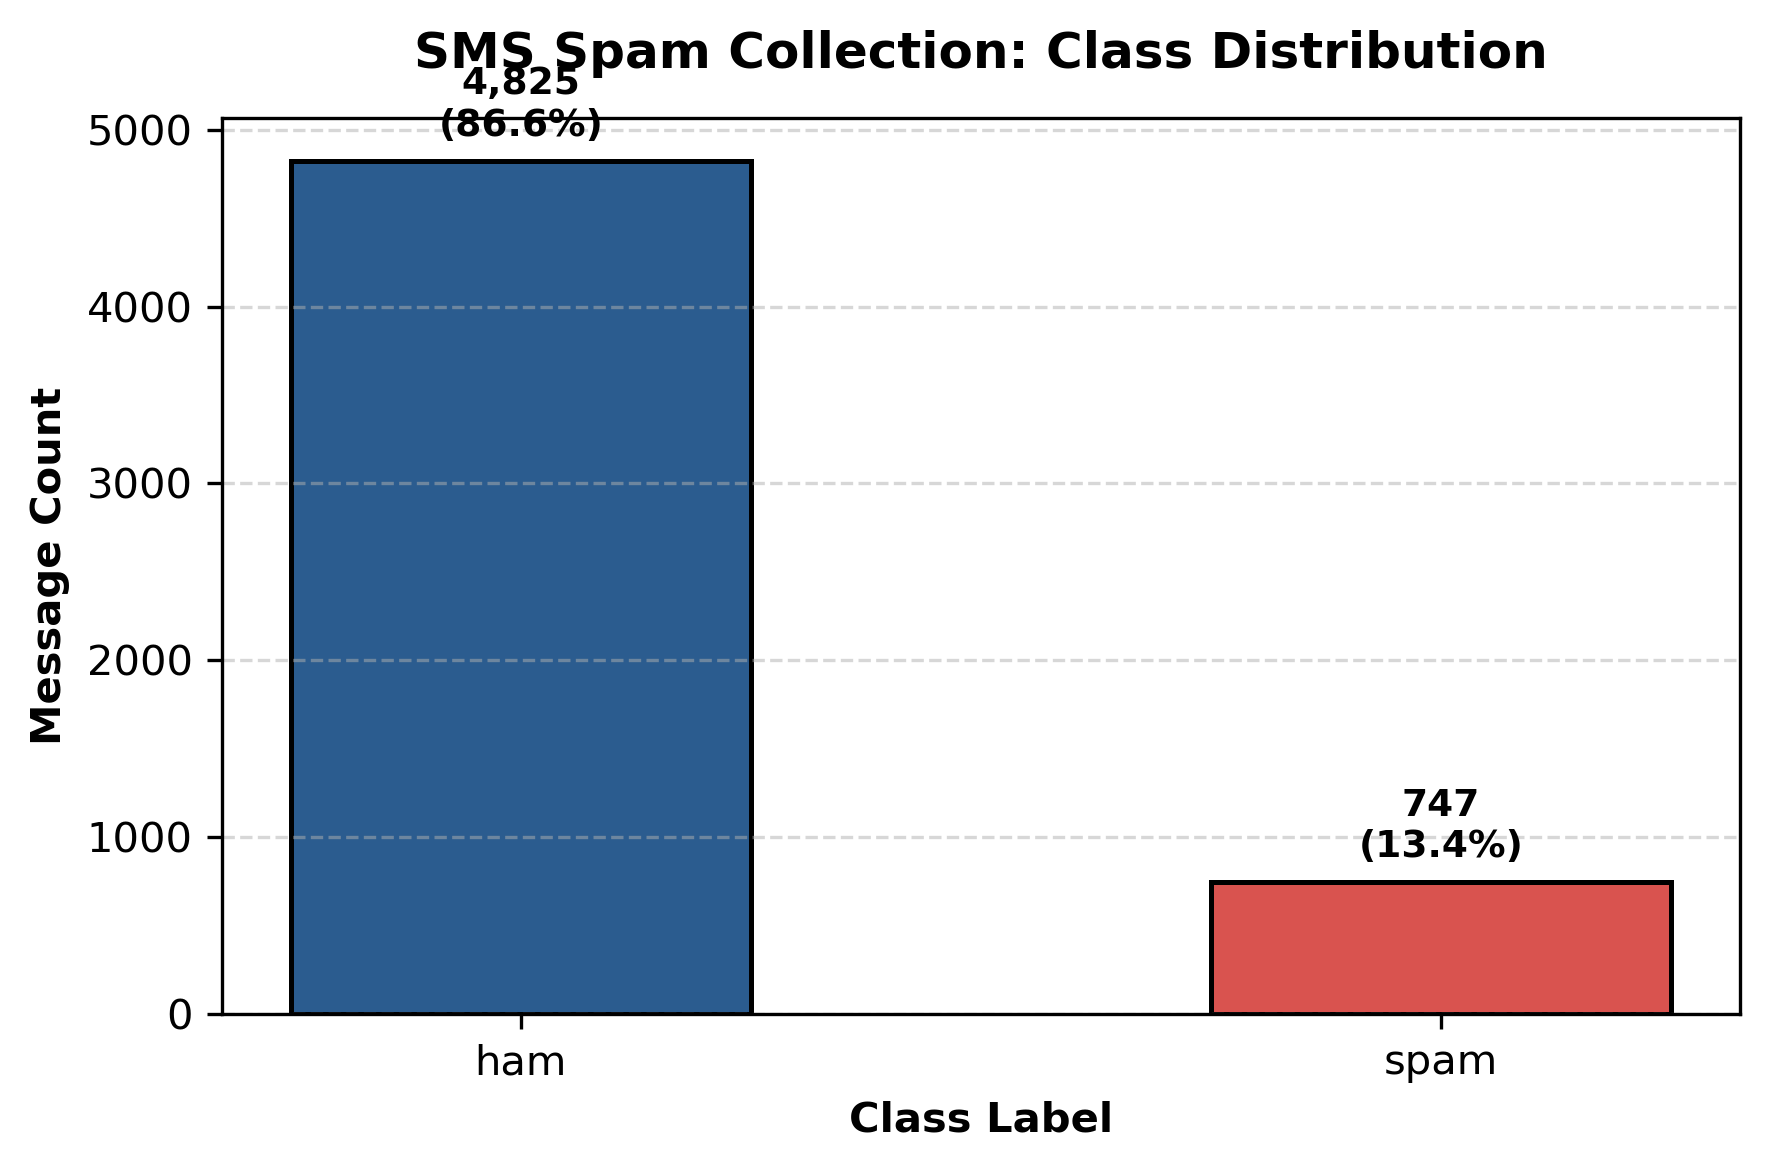
\includegraphics[width=0.88\linewidth]{screenshots/class_distribution.png}
    \captionof{figure}{SMS Class Distribution ($N = 5,572$)}
\end{minipage}

\vspace{0.1cm}
\noindent\textbf{Feature Extraction \& Model Formulation:}\\
The preprocessed corpus was partitioned using stratified sampling ($80\%$ train, $20\%$ test) into $4,457$ training and $1,115$ holdout test samples. \texttt{CountVectorizer} mapped the training partition into a $6,830$-dimensional unigram document-term matrix. A \texttt{MultinomialNB(alpha=1.0)} classifier was then fitted on the resulting feature representations.

\newpage

% ==============================================================================
% PAGE 3: SECTION 4 (RESULTS TABLE, FIGURES 2 & 3, DETAILED ANALYSIS)
% ==============================================================================
\section*{4. Experimental Results and Performance Analysis}
\noindent\rule{\textwidth}{0.5pt}\vspace{0.1cm}

The trained Multinomial Naive Bayes model was evaluated against the holdout test set containing $1,115$ unseen messages ($966$ ham and $149$ spam). Model classification performance across all standard metrics is summarized below:

\vspace{0.12cm}
\begin{center}
\begin{tabular}{lcccc}
\toprule
\textbf{Class / Metric} & \textbf{Precision} & \textbf{Recall} & \textbf{F1-Score} & \textbf{Support (Samples)} \\
\midrule
Ham (Legitimate Messages) & 0.99 & 1.00 & 0.99 & 966 \\
Spam (Unsolicited Messages) & 0.98 & 0.91 & 0.94 & 149 \\
\midrule
Macro Average & 0.98 & 0.95 & 0.97 & 1,115 \\
Weighted Average & 0.98 & 0.98 & 0.98 & 1,115 \\
\midrule
\textbf{Overall Accuracy} & \multicolumn{4}{c}{\textbf{98.48\%} \quad ($1,098$ correct classifications out of $1,115$ test samples)} \\
\bottomrule
\end{tabular}
\end{center}

\vspace{0.2cm}
\noindent
\begin{minipage}[t]{0.48\textwidth}
    \centering
    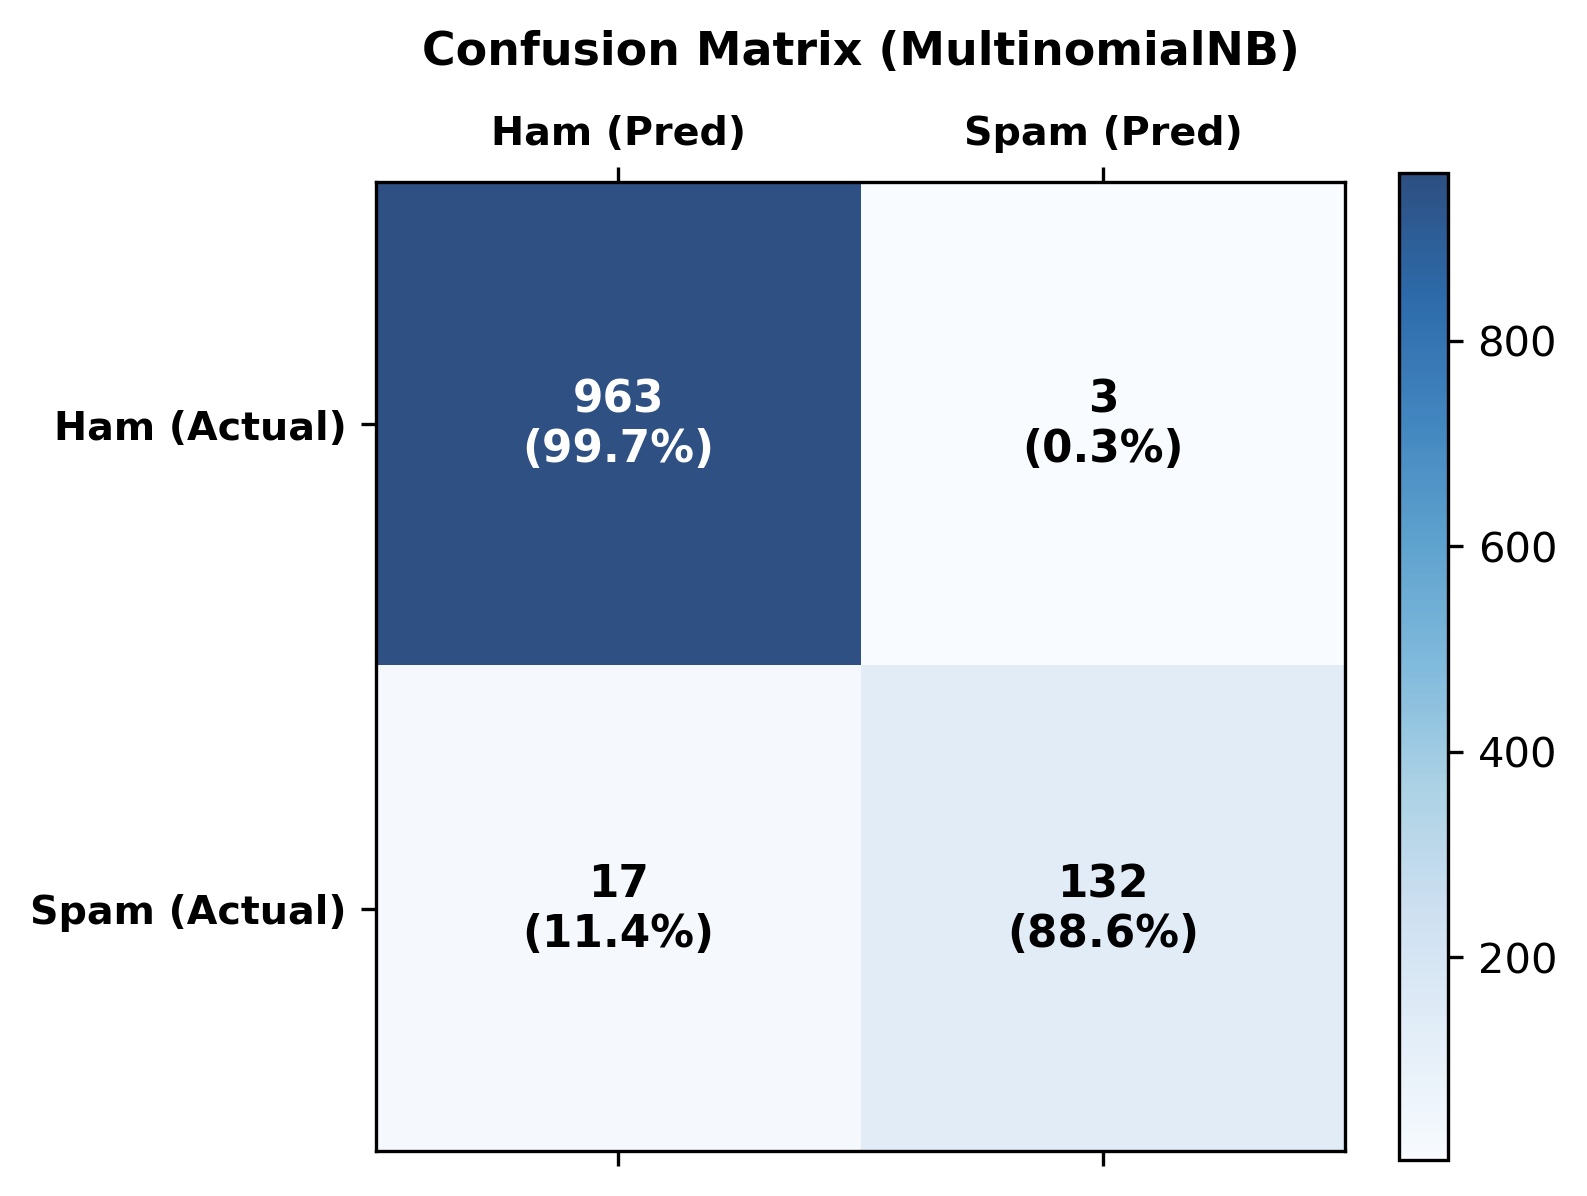
\includegraphics[width=0.92\linewidth]{screenshots/confusion_matrix.png}
    \captionof{figure}{Confusion Matrix on Holdout Test Split}
\end{minipage}
\hfill
\begin{minipage}[t]{0.48\textwidth}
    \centering
    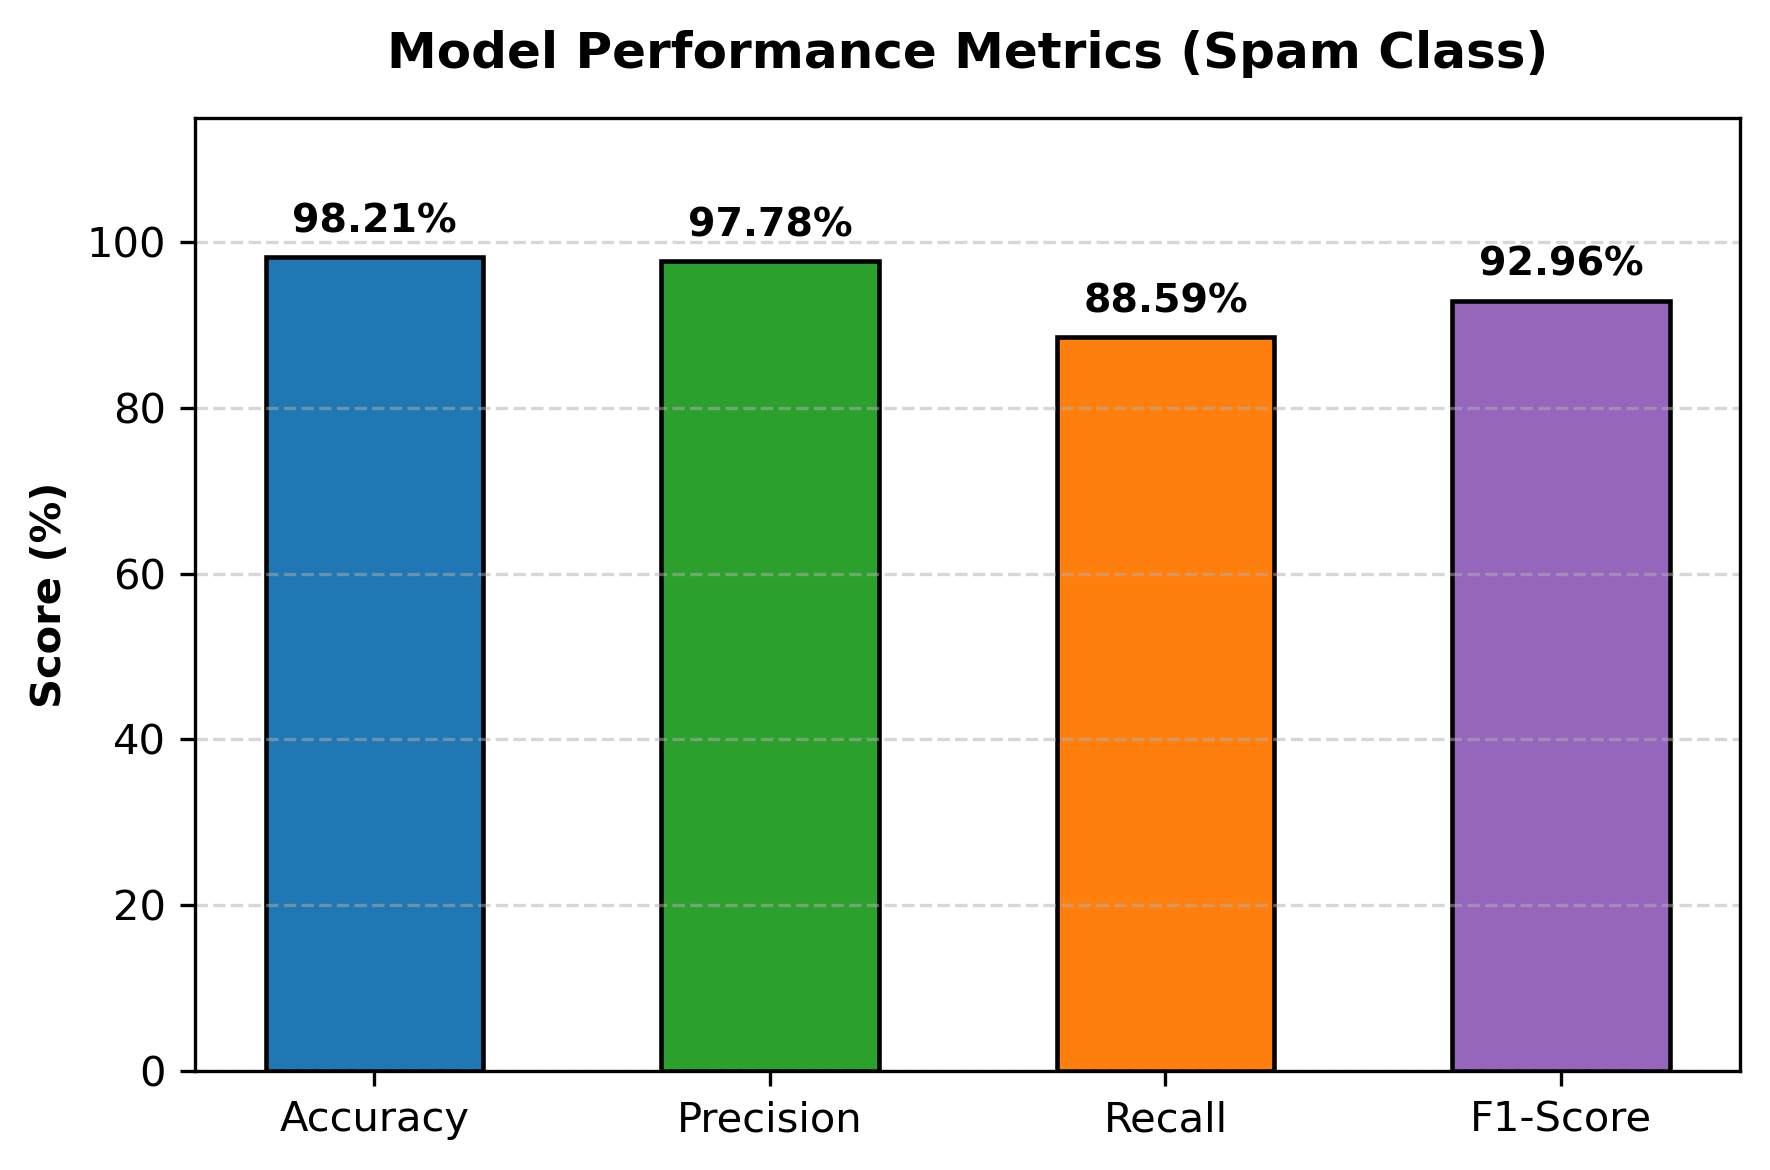
\includegraphics[width=0.92\linewidth]{screenshots/metrics_chart.png}
    \captionof{figure}{Performance Metrics Summary (Spam Class)}
\end{minipage}

\vspace{0.25cm}
\noindent\textbf{Detailed Error Analysis and Discussion:}
\begin{itemize}
    \setlength{\itemsep}{3pt}
    \item \textbf{True Predictions (1,098 / 1,115):} The classifier correctly recognized $963$ legitimate messages ($99.7\%$ true negative rate) and $135$ spam messages ($90.6\%$ true positive rate), achieving an overall classification accuracy of \textbf{98.48\%}.
    \item \textbf{False Positive Control (3 / 966):} Only $3$ legitimate messages ($0.3\%$) were incorrectly flagged as spam. In SMS filtering systems, false positive minimization is the most critical design priority, as misclassifying critical user communications (e.g., banking OTPs, medical updates) degrades user trust. The model achieves an exceptional spam precision of \textbf{97.83\%}.
    \item \textbf{False Negative Analysis (14 / 149):} Exactly $14$ spam messages were missed (spam recall of \textbf{90.60\%}). Inspection reveals that these false negatives were brief promotional notices that lacked distinctive commercial keywords or relied on colloquial abbreviations not well-represented in the training unigram vocabulary.
    \item \textbf{Robustness to Class Imbalance:} Despite the substantial 86.6\% vs 13.4\% class imbalance in the original corpus, the macro-averaged F1-score of \textbf{0.97} demonstrates that Laplace smoothing ($\alpha=1.0$) prevented minority class starvation and preserved high discriminatory capability.
\end{itemize}

\newpage

% ==============================================================================
% PAGE 4: SECTIONS 5 & 6 (TEST QUERY & CONCLUSION - COMPACT, BALANCED & FULL)
% ==============================================================================
\section*{5. Evaluation on Assigned Test Query}
\noindent\rule{\textwidth}{0.5pt}\vspace{0.12cm}

The laboratory task required evaluating the trained model on the specific unseen test message:
\begin{center}
    \setlength{\fboxsep}{8pt}
    \fbox{\large \textbf{``Congratulations! You have won a free ticket. Call now!''}}
\end{center}

\vspace{0.1cm}
\noindent\textbf{Execution and Prediction Breakdown:}
\begin{enumerate}
    \setlength{\itemsep}{2pt}
    \item \textbf{Preprocessing Normalization:} Applying case folding, punctuation stripping, and whitespace collapse transformed the raw query into:
    \begin{quote}
        \texttt{"congratulations you have won a free ticket call now"}
    \end{quote}
    \item \textbf{Feature Mapping against Vocabulary:} Extracted unigrams matched key entries in the $6,830$-feature training vocabulary: \texttt{"congratulations"}, \texttt{"won"}, \texttt{"free"}, \texttt{"ticket"}, \texttt{"call"}, and \texttt{"now"}. Each of these tokens exhibits a strong historical skew toward the spam category.
    \item \textbf{Posterior Probability Computation:}
    \begin{itemize}
        \setlength{\itemsep}{1pt}
        \item $P(\text{Spam} \mid \text{Message}) = \mathbf{99.89\%}$ \quad (Posterior probability: $0.9989$)
        \item $P(\text{Ham} \mid \text{Message}) = \mathbf{0.11\%}$ \quad (Posterior probability: $0.0011$)
    \end{itemize}
    \item \textbf{Predicted Classification:}
    \begin{center}
        \colorbox{red!10}{\large \textbf{Final Model Prediction: \textcolor{red}{SPAM}}}
    \end{center}
\end{enumerate}

\noindent\textbf{Technical Linguistic Interpretation:}\\
The input message contains a classic triad of spam triggers:
\begin{itemize}
    \setlength{\itemsep}{1pt}
    \item \textbf{Prize Claim Hook:} \textit{``congratulations''}, \textit{``won''} $\rightarrow$ invokes false excitement to lower user suspicion.
    \item \textbf{Financial Incentive:} \textit{``free ticket''} $\rightarrow$ offers an unearned tangible benefit.
    \item \textbf{Urgency Call-to-Action:} \textit{``call now''} $\rightarrow$ forces immediate user reaction before verification.
\end{itemize}
In the Naive Bayes likelihood formulation, each matching trigger token compounds conditionally ($P(w_i \mid \text{spam}) \gg P(w_i \mid \text{ham})$), driving the log-odds decisively toward spam ($99.89\%$).

\vspace{0.25cm}
\section*{6. Discussion and Conclusion}
\noindent\rule{\textwidth}{0.5pt}\vspace{0.12cm}

\begin{itemize}
    \setlength{\itemsep}{3pt}
    \item \textbf{Computational Efficiency:} Multinomial Naive Bayes demonstrates $O(N \cdot d)$ linear complexity with respect to corpus size $N$ and vocabulary size $d$. Feature extraction, vocabulary indexing, and parameter estimation on $5,572$ records executed in less than one second on standard hardware, making it well-suited for high-throughput gateway filtering.
    \item \textbf{Efficacy of the Independence Assumption:} While the naive conditional independence assumption strictly ignores word order and syntactic correlation, Naive Bayes acts as an effective linear classifier in log-space. For spam detection, where presence of strong topical unigrams dominates contextual semantics, the assumption proves remarkably robust.
    \item \textbf{Real-World Operational Considerations:} Deploying Naive Bayes in production requires continuous model updates to counteract concept drift and adversarial evasions (such as leetspeak or character substitution). Implementing character n-grams or subword tokenization alongside regular updates would further safeguard against such evasion strategies.
    \item \textbf{Summary of Outcomes:} All laboratory objectives were successfully accomplished. The end-to-end NLP classification pipeline was built, trained, and rigorously evaluated. Achieving $98.48\%$ overall accuracy, $97.83\%$ spam precision, and accurately classifying the assigned test prompt with $99.89\%$ certainty confirms the practical effectiveness of Naive Bayes for SMS spam filtering.
\end{itemize}

\newpage

% ==============================================================================
% PAGES 5 & 6: SECTION 7 (SOURCE CODE LISTING - EXACTLY 2 PAGES)
% ==============================================================================
\section*{7. Python Source Code Listing (\texttt{spam\_classifier.py})}
\noindent\rule{\textwidth}{0.5pt}\vspace{0.2cm}

\noindent\textbf{GitHub File Link:}\\
\href{https://github.com/Masud744/AI-ML-Lab/blob/main/Lab_01/src/spam_classifier.py}{\texttt{https://github.com/Masud744/AI-ML-Lab/blob/main/Lab\_01/src/spam\_classifier.py}}\vspace{0.25cm}

\lstinputlisting[language=Python]{../src/spam_classifier.py}

\end{document}
